\documentclass[11pt, oneside]{article}   	% use "amsart" instead of "article" for AMSLaTeX format
\usepackage{geometry}                		% See geometry.pdf to learn the layout options. There are lots.
\geometry{letterpaper}                   		% ... or a4paper or a5paper or ... 
%\geometry{landscape}                		% Activate for for rotated page geometry
%\usepackage[parfill]{parskip}    		% Activate to begin paragraphs with an empty line rather than an indent
\usepackage{graphicx}				% Use pdf, png, jpg, or eps§ with pdflatex; use eps in DVI mode
								% TeX will automatically convert eps --> pdf in pdflatex		
\usepackage{amssymb}
\usepackage{amsmath}

\title{Coring an apple}
%\author{The Author}
\date{}							% Activate to display a given date or no date

\graphicspath{{/Users/telliott_admin/Dropbox/Tex/png/}}

\begin{document}

\maketitle
\large
\noindent
In this short write-up I want to explore the use of polar coordinates to solve a problem of volume. This is the shape known as "the cored apple", shown in the figure (from Adams et al.).
\begin{center} 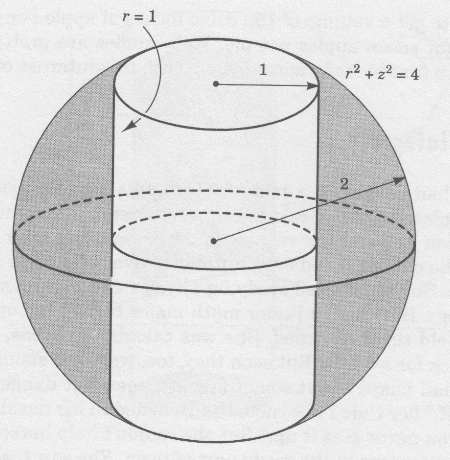
\includegraphics [scale=0.35] {apple_core.png} \end{center}
We have a sphere of radius $2$ which has had the central portion consisting of a cylinder plus the two spherical caps removed.  The cylinder has radius $1$.  We need to find the volume of the part that remains.

One way to do this problem is to find the volume of each spherical cap.  We worked this out in another short write-up.  
\begin{center} 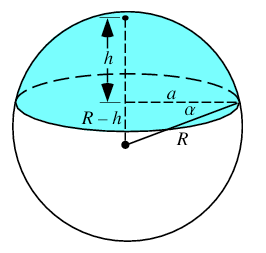
\includegraphics [scale=0.6] {spherical_cap.png} \end{center}
If $h$ is the height of the cap, then its volume is
\begin{equation}
\boxed{V_{cap} = \frac{1}{3} \pi h^2(3R - h)}
\end{equation}
We are given $r$, which is labeled $a$ in the second figure.  The equation we get using the Pythagorean theorem is
\[ R - h = \sqrt{R^2 - r^2 } = \sqrt{3} \]
\[ h = 2 - \sqrt{3} \]
\[ h^2 = 7 - 4 \sqrt{3} \]
So the volume of one spherical cap is
\[ V = \frac{1}{3} \pi (7- 4 \sqrt{3})(6-(2-\sqrt{3})) \]
\[ = 16 - 9 \sqrt{3} \]
We have two of these
\[ V = 2(16 - 9 \sqrt{3}) \]
The volume of the cylinder is the area of the cross-section ($\pi$) times the height, which is twice $R-h$.
\[ V = 2 \pi \sqrt{3} \]
We have to subtract both of these from the volume of the whole sphere, which is $32/3 \pi$.  The desired quantity is
\[ \frac{32}{3} \pi - 2 \pi \sqrt{3} - 32 + 18 \sqrt{3} \]
I get
\[  33.5103 - 10.8828 - 32 + 32.1769 =   21.8044 \]
Just grind through it and we get there.
\vspace{5 mm}

\noindent
There is a more elegant approach, using calculus.  Consider the sphere as a surface above the circle.  For the circle we have $x^2 + y^2 = r^2$, where now we are using $r$ as a \emph{variable} that could range from $0 \rightarrow R$.

In Cartesian coordinates the circle is
\[ x^2 + y^2 + z^2 = R^2 \]
Using polar coordinates for $x$ and $y$ we have 
\[ r^2 + z^2 = R^2 \]
\[ z = \sqrt{R^2 - r^2} = \sqrt{4 - r^2}  \]
We will do a double integral over the the $xy$-plane, adding up the value of this function for each small area element $dA$.  In polar coordinates, the area element is
\[ dA = r dr d \theta \]
so, for example, the basic area integral is
\[ A = \int dA = \int_{\theta=0}^{2 \pi} \int_{r=0}^R r dr d \theta = \int_{\theta=0}^{2 \pi} \frac{1}{2}R^2 d \theta = \pi R^2 \]
Now, what we want is to integrate the surface height over the whole area, plugging in from above we get
\[ V = \int dV = \int_{\theta=0}^{2 \pi} \int_{r=0}^R \sqrt{R^2 - r^2}  \ r dr d \theta \]
This integral is not hard to do because we have the derivative of what is under the square root sign.  Let $u = R^2 - r^2$.  Then
\[ du = -2r dr \]
\[ -\frac{1}{2} du = r dr \]
so the inner integral is
\[ \int -\frac{1}{2} \sqrt{u}\  du = -\frac{1}{3} u^{3/2} \]
Substituting back, the inner integral (for the whole sphere) is 
\[ -\frac{1}{3} (R^2 -r^2)^{3/2} \bigg{|}_0^R = \frac{1}{3}(R^2)^{3/2} =  \frac{1}{3} R^3 \]
When we do the outer integral we pick up an extra factor of $2\pi$, which gives the correct value for the volume of the bemisphere.
What is great about this approach is that we don't have to start at $r=0$.  This simplifies our problem enormously.  In the problem, we start from $r=1$ (and we have $R=2$).  So this gives the volume we seek as
\[ V = \int dV = \int_{\theta=0}^{2 \pi} \int_{r=1}^2 \sqrt{4 - r^2}  \ r dr d \theta \]
The inner integral is
\[ -\frac{1}{3} (4 -r^2)^{3/2} \bigg{|}_1^2 = \frac{1}{3}(3)^{3/2} =  \sqrt{3} \]
Now we have
\[ V =  \int_{\theta=0}^{2 \pi} \sqrt{3} \ d \theta \]
which is just $2\pi \sqrt{3}$.  Times $2$ for the whole apple, we get
\[ 4 \pi \sqrt{3} = 21.7656 \]
Close enough for me.
\vspace{10 mm}

\noindent
Adams, Thompson and Hass.  \emph{How to Ace the Rest of Calculus}





\end{document}  